\subsection{Travail réalisé}\label{sec:work_done}
Nous avons vu dans dans la Figure \ref{frame_safe} le chemin suivi pour la création et la définition des \textit{Epics}, \textit{Millestones} et le \textit{Backlog}. Dans la Figure \ref{fig:backlog} nous pouvons regarder un exemple du contenu Backlog.

Pendant le déroulement de mon alternance, j'ai travaillé sur plusieurs items du \textit{Backlog}. Appendice  \ref{appen:my_backlog}. Chaque item était bien découpé de sorte que la tâche puisse se terminer dans le délai d'un \textit{Sprint}.

\begin{figure}[!ht]
\centering
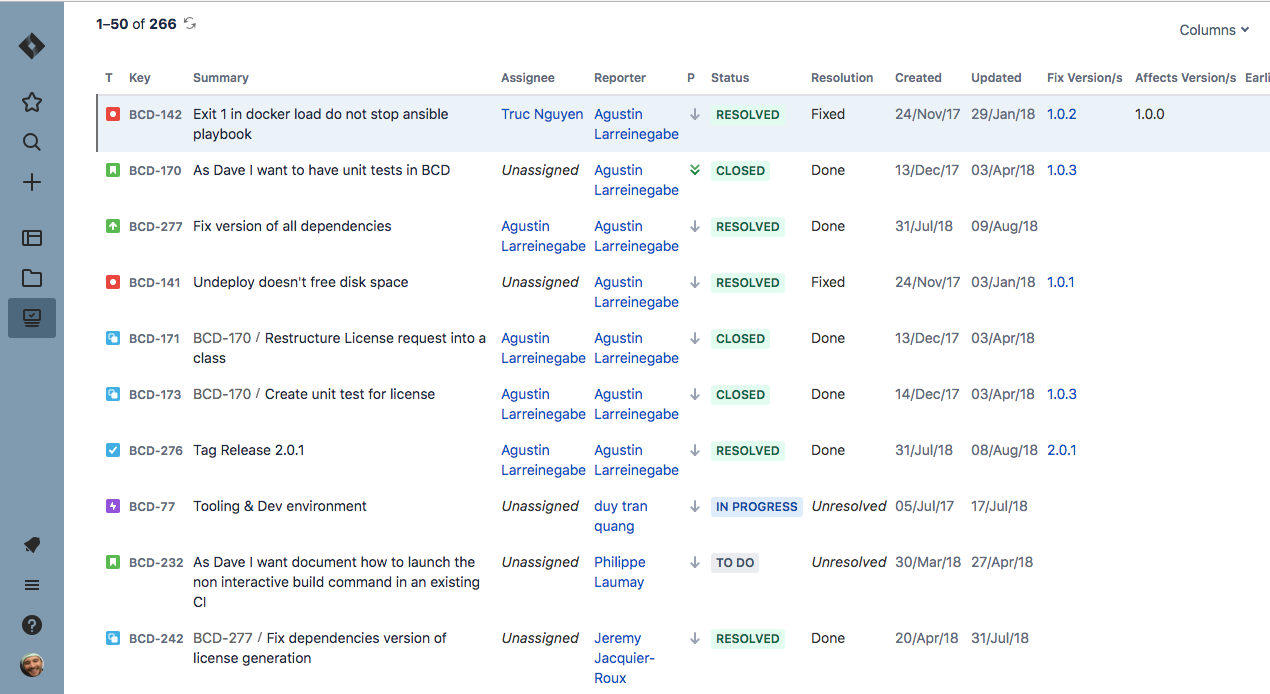
\includegraphics[width=\textwidth,keepaspectratio]{backlog.png}
\caption{Exemple Backlog}
\label{fig:backlog}
\end{figure}

Pour cela, je devais effectuer des actions différentes comme:

\subparagraph{Python} Développer et maintenir les scripts du Command Line Interface (CLI) de BCD.
\begin{itemize}
  \item J'ai participé à la réorganisation du code pour le rendre plus modulaire.
  \item J'ai participé à l'élaboration des tests unitaires pour le module BCD.
  \item J'ai participé au développement du module de \enquote{Licensing}.
\end{itemize}

\subparagraph{AWS} Une partie de BCD gère des instances dans le cloud, aussi l'entreprise a passé d'autres services sur le cloud.
\begin{itemize}
  \item J'ai aidé à implémenter le service \enquote{Organization} de AWS.
  \item J'ai dû m'impliquer plus dans les services EC2, Lambda, S3, RDS.
\end{itemize}

\subparagraph{Ansible} Développer et maintenir des \enquote{Playbook} Ansible.
\begin{itemize}
  \item J'ai participé à l'adaptation des scripts pour supporter le nouveau dépôt privé d'images docker.
\end{itemize}

\subparagraph{Jenkins} Exécution de jobs pour l'empaquetage de livrables.

\subparagraph{Git} Gestion du dépôt privé.
\begin{itemize}
  \item Revue de \enquote{Pull Request}
  \item \enquote{Merge} dans la branche correspondante.
  \item \enquote{Tag} et livre des nouvelles versions.
\end{itemize}

\subparagraph{Docker} Maintenir des images et l'investigation des nouvelles caractéristiques.

\subparagraph{Activités collatérales} Pour mieux organiser le travail en équipe, nous suivons des rituels Agile
\begin{itemize}
  \item Le \enquote{Daily Meeting} pour faire le point sur les tâches effectuées et communiquer sur les difficultés rencontrées.
  \item La \enquote{Rétrospective}, pour s’améliore.
  \item La \enquote{Réunion hebdomadaire},  elle réunit toutes les parties prenantes du projet pour faire le point sur son avancement. Ainsi, tous les participants peuvent se rendre compte si l’état du projet correspond à leurs besoins, attentes ou objectifs.
  \item \enquote{Les estimations}, où nous faisons des hypothèses à échelle relative, pour estimer une charge de travail par exemple. Cette réunion est importante pour déterminer correctement la complexité et la valeur apportée de la tâche à réaliser pour effectuer une estimation de bonne qualité.
  \item \enquote{La sélection}, où nous déterminons efficacement la charge de travail à accomplir définie dans le backlog lors de l'itération.
\end{itemize}

\subsubsection{Gestion de risques}
Il y a toujours plusieurs risques associés au développement du logiciel. Dans cette sous-partie, nous allons voir quelques risques que j'ai vu s'atténuer en comparaison à d'autres expériences de travail (pas Agile). \cite{basile_plessis_2014}
\begin{center}
\begin{tabular}{p{3cm}|p{3cm}|l|l|p{5cm}}
Description & Conséquence & Probabilité & Impact & Action \\ \hline
Prévision de travail pas juste & Rien livrer du tout & Faible & Fort & Le \enquote{Daily Metting} permet de s'assurer que sa prévision de \enquote{Sprint} est toujours d'actualité \\
Baisse de qualité du code & Bogue introduit & Modéré & Fort & Mise en place de CI, revues de code avant de l'ajouter dans la branche principale, test unitaire \\
Perte d'engagement de l'équipe & Équipe démotivée, et baisse de performance & Faible & Fort & La \enquote{Retrospective} suite de chaque \enquote{Sprint} aide l'équipe à s'améliorer. \\
Incompréhension des fonctionnalités & Ne pas livrer les bonnes fonctionnalités ou celles qui n'apportent pas de valeur & Faible & Modéré & Le \enquote{Spring Planning} permet à l'équipe de choisir les \enquote{stories} et s'engager. \\


\end{tabular}
\end{center}
